% !TEX root = ../Thesis.tex
\chapter{Testing with Trap-Driven Simulation}

Because superpage overlays require hardware changes, they can only be tested in a simulated system. To allow us to simulate superpage overlays in real time on real workloads, we use a system called trap-driven simulation \cite{Talluri}. This involves modifying the Linux kernel to keep track of a simulated TLB while running, and forcing a page fault to occur on every memory access that would be a miss in the simulated TLB. Thus, the simulation can be updated accurately.

An existing testing system called BadgerTrap \cite{BadgerTrap} was used as the basis of our infrastructure. BadgerTrap measures real TLB misses by a method similar to trap-driven simulation. Each page table entry has a section of ``reserved'' bits, which are not supposed to be touched by the kernel. When the MMU sees a reserved bit set during a page table walk, it immediately page faults with a specific error code. BadgerTrap takes advantage of this by setting a reserved bit on every page in the address space of the process being tested. Then, whenever there is a TLB miss the resulting page table walk causes a distinctive page fault, which BadgerTrap records. It proceeds to unset the reserved bit, read the address to get it into the TLB, and sets the reserved bit again so the next TLB miss will have the same result.

We ported BadgerTrap to the latest version of the Linux kernel and modified it to simulate a TLB. Every time an address is replaced in the simulated TLB, it is flushed from the real TLB as well so that every access that would be a miss in the simulation is also a miss in the real TLB. That allows the simulation to remain accurate and work exactly the same as if it were a real system, and the performance impact is minimal since it only does any work on TLB misses.

Trap-driven simulation works as long as TLB misses are the only time any updates need to happen. The only thing this limits significantly is the replacement policy. We use a variant of ``not recently used'' (NRU), where a bit is set whenever the page is accessed, by also clearing pages from the real TLB if their ``used'' bit is 0 so that it can be updated on their next access. Pages with a 0 ``used'' bit are replaced first, and if all pages have it set then all the ``used'' bits are cleared and the first page is replaced.

\section{Benchmark}
The main benchmark for measuring the effectiveness of superpage overlays is a fork-write program. It simply allocates 2MB of memory as either one superpage or many regular pages, forks, and the child process writes to the whole memory region or only the first few bytes. This triggers one or more copy-on-write, and the performance depends on how many TLB misses occur during the writes and how much data is copied. Figure \ref{fig:charts} shows the average time and TLB misses for the different configurations of the benchmark, measured by the Linux perf tool. This benchmark demonstrates the potential for superpage overlays to improve performance. Writing to many 4KB pages is slow due to the high number of TLB misses, but doing copy-on-write with a superpage is slow compared to the 4KB pages when the writes only affect a small amount of memory. Superpage overlays should provide the TLB benefits of superpages while only copying 4KB at a time when the child process writes.

So far, the trap-driven simulation can effectively simulate a normal TLB without overlays. Figure \ref{fig:tables} shows simulated TLB misses vs real TLB misses measured by the perf tool. The first graph is from running a variety of arbitrary Linux utilities like grep and cat. It shows that, while the simulated TLB behaves differently due to only storing translations for a single process and not including kernel memory, it generally correlates with the real TLB and anything that reduces simulated misses is likely to have real-world benefit. The second graph is from running the fork-write benchmark multiple times in a loop. The completely linear relationship shows that the benchmark is consistent and reliable, which makes it a good simple model on which to test overlays.
\begin{figure}
    \centering
    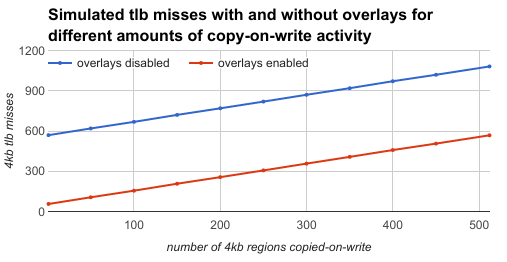
\includegraphics[width=3in]{Figures/Graph1}
    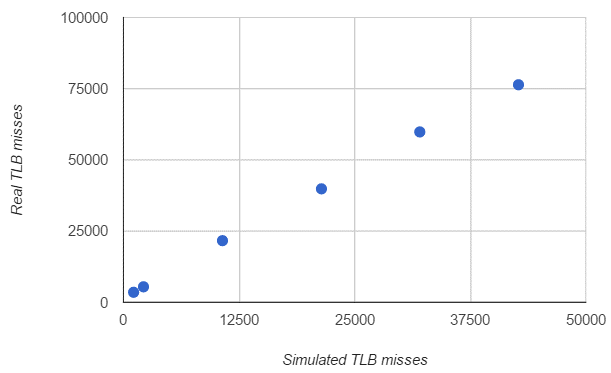
\includegraphics[width=3in]{Figures/Graph2}
    \caption{Simulated vs. real TLB misses on different workloads}
    \label{fig:charts}
\end{figure}

\begin{figure}
    \centering
    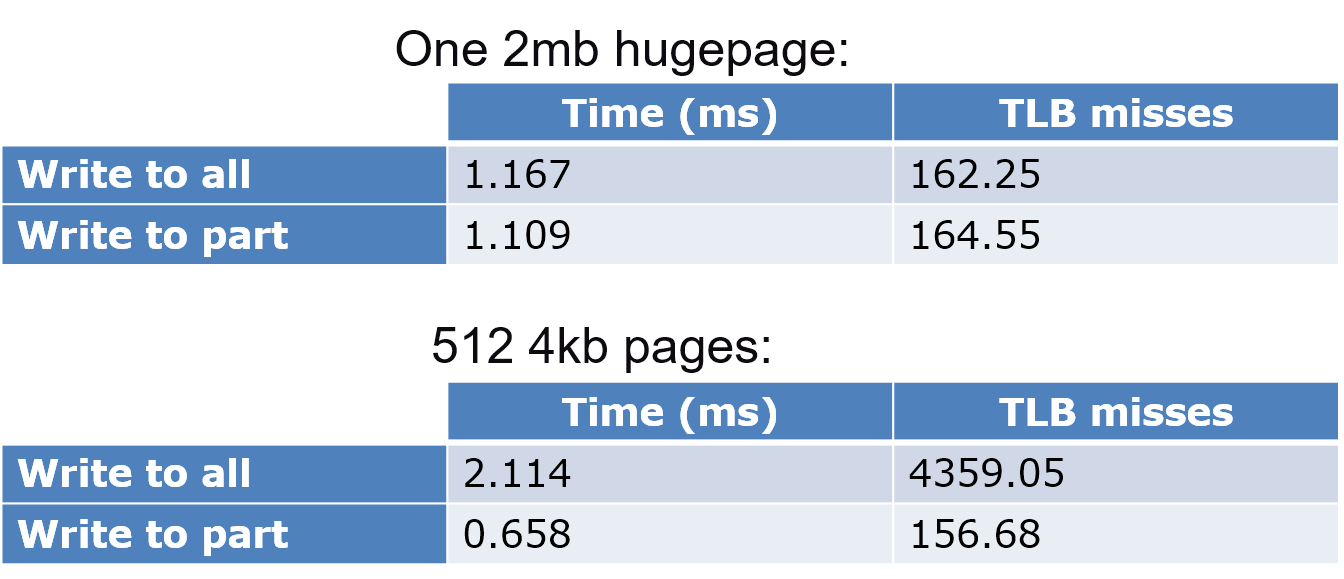
\includegraphics[width=3.2in]{Figures/Table1}
    \caption{Real TLB misses and elapsed time for the 4 different configurations of the fork-write benchmark}
    \label{fig:tables}
\end{figure}
